\documentclass[10pt]{article}
\usepackage{amsmath}
%encoding
%--------------------------------------

%----------------------------
\usepackage{microtype}
%\usepackage{fourier}
\usepackage{lmodern}
\renewcommand{\familydefault}{\sfdefault}

\usepackage[utf8]{inputenc}
\usepackage[T1]{fontenc}

%units
%--------------------------------------
\usepackage{siunitx}
%drawing
%------------------------------------
\usepackage{tikz} % To generate the plot from csv
\usepackage{pgfplots}
\usepackage{pgfplotstable}
\usepackage{graphicx}

\usepackage{caption}
\usepackage{color, colortbl}
\usepackage{tabularx}
\usepackage{setspace}
\usepackage{mhchem}
\usepackage{fancyhdr}
\pagestyle{fancy}

\cfoot{\thepage}

\rhead{\footnotesize Gruppe 24}
\lhead{\footnotesize Titration der starken Säure - Starken Base}
\setlength{\headheight}{15pt}
\makeatletter
\setlength{\@fptop}{0pt}
\makeatother

\renewcommand{\familydefault}{\sfdefault}
\captionsetup{font=footnotesize}

\definecolor{LightCyan}{rgb}{0.88,1,1}
\usetikzlibrary{datavisualization}
\pgfplotsset{compat=newest} % Allows to place the legend below plot
\usepgfplotslibrary{units} % Allows to enter the units nicely
\usepackage{overcite}
\renewcommand\citeform[1]{[#1]}

\sisetup{
  round-mode          = places,
  round-precision     = 2,
  inter-unit-product =\ensuremath{{}\cdot{}}
}

%\usetikzlibrary{arrows, positioning, calc, datavisualization}


\usepackage{url}

\begin{document}
%\begin{luacode*}
function string:split(sep)
        local sep, fields = sep or "%s", {}
        local pattern = string.format("([^%s]+)", sep)
        self:gsub(pattern, function(c) fields[#fields+1] = c end)
        return fields
end

function printHyperbola()
    local lines={}

    for line in io.lines("dampf.csv") do
            table.insert(lines, line)
    end
    tex.sprint("\\addplot[color=black] coordinates{")

    for i=2,#lines do
        local a=lines[i]:split()
        tex.sprint("("..a[1]..","..a[2]..")")
    end
     tex.sprint("};")
    tex.sprint("\\addplot[color=blue] coordinates{")

    for i=2,#lines do
        local a=lines[i]:split()
        tex.sprint("("..a[1]..","..a[3]..")")
    end
     tex.sprint("};")

end
\end{luacode*}
%\begin{figure}
\centering
     \begin{tikzpicture}
            \begin{axis}[standard,xlabel=Temperatur,ylabel=Druck]
                \directlua{printHyperbola()}
            \end{axis}
        \end{tikzpicture}
     \end{figure}
\tikzset{every mark/.append style={scale=0.6}}
\begin{figure}
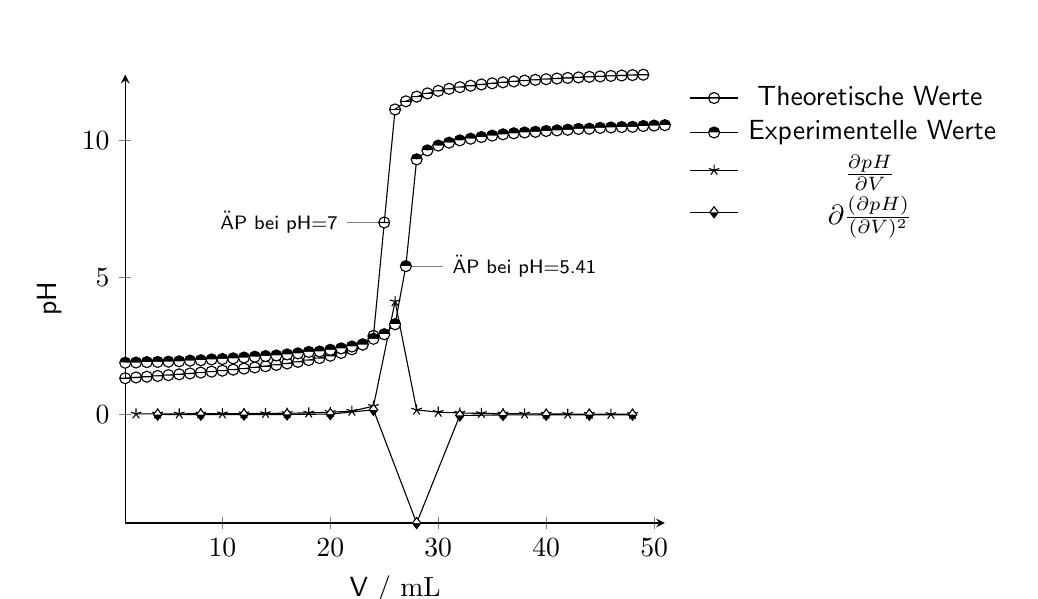
\begin{tikzpicture}
\begin{axis}[
axis equal=false,
axis x line=bottom,
axis y line=middle,
legend style={draw=none,legend pos=outer north east},
xlabel= \ce{V} / \si{\milli\liter},
ylabel= pH,
y label style={at={(axis description cs:-0.1,.5)},rotate=90,anchor=south}
]
\addplot[mark=halfcircle] table{
X Y
1 1.3273589343863
2 1.3542755076172
3 1.3818531887786
4 1.410174465089
5 1.4393326938303
6 1.4694344260534
7 1.5006023505692
8 1.5329790721847
9 1.5667320289862
10  1.602059991328
11  1.6392017993325
12  1.6784483371914
13  1.720159303406
14  1.7647872888257
15  1.8129133566429
16  1.8653014261025
17  1.9229848157089
18  1.987410872692
19  2.0606978403536
20  2.1461280356782
21  2.2491983573911
22  2.3802112417116
23  2.5622928644565
24  2.869231719731
25 7
26  11.119186407719
27  11.414539270491
28  11.585026652029
29  11.704432900038
30  11.795880017344
31  11.869666231505
32  11.931284187631
33  11.984011894616
34  12.029963223377
35  12.070581074286
36  12.106894233915
37  12.139661993429
38  12.169460680157
39  12.196738029033
40  12.221848749616
41  12.245078590335
42  12.266661094033
43  12.286789556549
44  12.305625747353
45  12.323306390375
46  12.339948061694
47  12.355650946556
48  12.370501760325
49  12.384576047114
};
\node[coordinate,pin=left:{\scriptsize ÄP bei pH=7}]
at (axis cs:25,7) {};
\node[coordinate,pin=right:{\scriptsize ÄP bei pH=5.41}]
at (axis cs:27,5.41) {};
\addlegendentry{Theoretische Werte}
\addplot[mark=halfcircle*] table {
  X Y c
  1 1.891272523 0
2 1.898857874	0.1
3 1.914028575	0.2
4 1.921613925	0.3
5 1.929199276	0.4
6 1.944369977	0.5
7 1.967126029	0.6
8 1.982296731	0.7
9 2.012638133	0.8
10 2.027808834	0.9
11 2.050564886	1
12 2.080906289	1.1
13 2.111247691	1.2
14 2.134003743	1.3
15 2.156759795	1.4
16 2.194686548	1.5
17 2.232613302	1.6
18 2.285710756	1.7
19 2.300881457	1.8
20 2.361564262	1.9
21 2.414661717	2
22 2.482929873	2.1
23 2.551198028	2.2
24 2.763587846	2.3
25 2.93046556	2.4
26 3.294562391	2.5
27 5.410875219	2.6
28 9.302160095	2.7
29 9.628330173	2.8
30 9.802793237	2.9
31 9.908988146	3
32 9.992427003	3.1
33 10.05310981	3.2
34 10.11379261	3.3
35 10.16689007	3.4
36 10.21240217	3.5
37 10.25032893	3.6
38 10.28067033	3.7
39 10.30342638	3.8
40 10.33376778	3.9
41 10.35652383	4
42 10.37927989	4.1
43 10.40962129	4.2
44 10.41720664	4.3
45 10.44754804	4.4
46 10.46271874	4.5
47 10.47788944	4.6
48 10.48547479	4.7
49 10.5158162	4.8
50 10.5309869	4.9
51 10.5461576	5
};
\addlegendentry{$\,$Experimentelle Werte}
\addplot[mark=star] table {
X Y
2 0.0269165732309
4 0.0283212763104
6 0.0301017322231
8 0.0323767216155
10  0.0353279623418
12  0.0392465378589
14  0.0446279854197
16  0.0523880694596
18  0.0644260569831
20  0.0854301953246
22  0.1310128843205
24  0.3069388552745
26  4.119186407719
28  0.170487381538
30  0.091447117306
32  0.061617956126
34  0.045951328761001
36  0.036313159629
38  0.029798686728
40  0.025110720583001
42  0.021582503697999
44  0.018836190804
46  0.016641671319
48  0.014850813769
};
\addlegendentry{ $\frac{\partial pH}{\partial V}$ }
\addplot[mark=halfdiamond*] table {
X Y
4 0.0014047030794999
8 0.0022749893923999
12  0.0039185755170998
16  0.0077600840399001
20  0.0210041383415
24  0.175925970954
28  -3.948699026181
32  -0.02982916118
36  -0.0096381691320016
40  -0.0046879661449992
44  -0.0027463128939988
48  -0.0017908575500005
};
\addlegendentry{ $\partial \frac{(\partial pH)}{(\partial V)^2}$}

\end{axis}

\end{tikzpicture}
\caption{Säure-Base-Titration }
\end{figure}
%\ce{H2SO4 + 2NaOH -> Na2SO4 + 2H2O}
\end{document}

%%\addplot[domain=0:1200]{-1.42e-5*x^(2)+2.836e-2*x+45.47};

